\documentclass[12pt, twoside]{report}

%Packages
\usepackage{setspace} %for onehalf spacing
\usepackage{graphicx} %for includegraphics
\usepackage{float} %for H pointer in graphics
\usepackage{titlesec} %to make section titles smaller
%Required packages in csfyp class:
\usepackage[top=1.2in, left=2.7cm, bottom=1.2in, right=2.7cm]{geometry} 
\usepackage{calc}
\usepackage[bottom]{footmisc}
\usepackage{caption}
\captionsetup[table]{skip=1ex}

%Parameters
\onehalfspacing
\renewcommand\thesection{\arabic{section}} %change numbering style of sections
\titleformat*{\section}{\large\bfseries}
\titleformat*{\subsection}{\small\bfseries}

\begin{document}
	%Title Page:
	\begin{titlepage}
		\centering
		{\LARGE\bfseries Machine learning for data mining and performance optimization at the CERN Large Hadron Collider \par}
		\vspace{.5cm}
		
		{\Large \textbf{Progress Report} \par}
		\vspace{.5cm}
		
		{\large \textbf{Marc Ferriggi}\par}
		\vspace{0.5cm}
		
		{\large \textbf{Supervisor:} Dr. Gianluca Valentino\par}
		\vfill
		
		
\includegraphics[width=0.65\textwidth]{UoMLogo}\par
		\vfill
		
		{\large\bfseries Faculty of Science \par}
		{\large\bfseries University of Malta \par}
		{\large\bfseries December 2018 \par}
		
		\vspace{1cm}
		\textit{Submitted in partial fulfillment of the requirements for the degree of B.Sc. (Hons.) Computing Science AND Statistics and Operations Research}
	\end{titlepage}
	
	\tableofcontents
	\pagebreak
	
	\section{Abstract}
	\paragraph{ }The CERN particle accelerator complex generates around 2 TB of data per week from almost 1 million signals. In this dissertation, unsupervised machine learning techniques for applications such as clustering and anomaly detection shall be used to analyse past LHC data in order to visualize correlations, determine data driven models and identify opportunities for improving the LHC machine availability and performance reach.
	
	\section{Introduction \& Motivation}	
	\paragraph{ }The LHC is filled to flat top intensity by injecting each beam with kicker waves 12 times \cite{r:BeamQC}. This is a challenging task given the high energy of the beam, the very small apertures and the delivery precision's tight tolerances, thus multiple sensors are installed around the CERN particle accelerator complex \cite{r:Diagram} which gather readings and data that can be used to check the quality of the injected beam. This data is stored using CERN's LS (Logging Service). The LS is heavily used and in 2013, it was noted that close to 1000 users relied on it \cite{r:LS}. While many studies have been made using this logged data and lots of statistical tests have been done with regards to injection quality checks for the LHC (such as \cite{r:AutomaticIQCChecks} and \cite{r:BeamQC}), no studies can be found on the CERN Document Server \cite{r:CERNDocumentServer} where researchers used unsupervised machine learning methods to analyse this data.
	\par The purpose of this thesis is to go through the entire process in a data science project and learn to use unsupervised machine learning techniques for applications such as clustering and anomaly detection. These techniques will then be used to analyse past LHC data in different machine configurations to visualise correlations, determine data-driven models and identify opportunities for improving the LHC machine availability and performance reach in terms of beam lifetime, beam stability and luminosity.
	
	\section{Why is the Problem non-Trivial}
	
	\paragraph{ }The LS currently generates around 2 TB of data per week. This data is generated from multiple machines each measuring different features of the waves at different points in the accelerator complex. Thus the data must be thoroughly analysed and normalised in order to be able to apply the machine learning analysis techniques properly. Identifying opportunities to improve the beam lifetime, beam stability and luminosity is also a non-trivial problem to tackle.
	
	
	\section{Background Research and Literature Review}
	\subsection{Unsupervised Machine Learning Techniques}
	\paragraph{ }Unsupervised machine learning algorithms refer to the class of machine learning algorithms where the observations only are available to the learner as there is no access to a training set or the aim of the algorithm is simply to observe patterns in these observations. In fact, A. Hyv{\"a}rinen states in \cite{r:lecturenotes} that for unsupervised learning ``(w)e don't have separate ``inputs" and ``outputs", just a lot of observations of one variable or vector". Hyv{\"a}rinen continues to state some goals of unsupervised learning which include data visualisation, noise reduction, feature extraction and finding interesting components, which are all of particular interest for this study.
	\par The following points are a summary of the research made on some of the unsupervised machine learning algorithms that will be used in this study:
	\begin{itemize}
		\item \textit{K-Means Clustering}: K-Means is considered to be one of the most popular clustering methods \cite{r:jin}. The idea behind the algorithm is to split the data into $k$ clusters where a data point forms part of the cluster with the closest centroid. The time complexity for this algorithm is $O(nki)$ and the space complexity is $O(n(d+k))$ where $n$ is the number of points, $k$ the number of centres, $d$ the number of dimensions and $i$ the number of iterations required to converge \cite{r:jin}. 
		\item \textit{DBSCAN}: This algorithm was created from the necessity of having a clustering algorithm with the following requirements:
		\begin{enumerate}
			\item ``Minimal requirements of domain knowledge to determine the input parameters,"
			\item ``Discovery of clusters with arbitrary shape," and
			\item ``Good efficiency on large databases" \cite{r:DBSCAN}
		\end{enumerate}
		DBSCAN manages to attain the above requirements by viewing clusters as ``areas of high density separated by areas of low density" \cite{r:skclustering}. This algorithm also introduces the concept of \textit{core samples} which was then used in the designing of other machine learning algorithms such as LOF (Local Outlier Factor).
		\item \textit{Local Outlier Factor}: The LOF refers to a ``degree of outlier-ness" that this algorithm considers for each point in the data rather than using the concept that ``being and outlier is binary" \cite{r:LOF}. This algorithm uses a clustering technique which takes concepts from DBSCAN to measure the LOF of each point where an LOF value $>1$ implies that the point has lower density than its neighbours and is thus probably an outlier. 	
	\end{itemize}
	
		
	\subsection{Choosing a Python Package}
	\paragraph{ }Although performance of k-means and k-Nearest Neighbours is not as optimal as in other Python packages (such as `\textit{PyMVPA}' \cite{r:pymvpa} or `\textit{shogun}' \cite{r:shogun}), it was decided to use the `\textit{scikit-learn}' machine learning package for this thesis due to its ``state-of-the-art implementation" and ``easy-to-use interface tightly integrated with the Python language" \cite{r:sklearn}. Furthermore, the algorithms implemented using this package can be ``used as building blocks for approaches specific to a use case" \cite{r:sklearn} which will be useful if one would like to extend the scope of this thesis.
	
	
	%\section{Aims and Objectives}
	%\paragraph{ }The aim of this project is to utilise unsupervised machine learning algorithms to analyse past LHC data with the hopes of identifying opportunities to improve the LHC machine availability and performance reach in terms of beam lifetime, beam stability and luminosity.
	
	\section{Methods and Techniques Used or Planned}
	\subsection{The Parameters Studied}
	\paragraph{ }In this subsection, the data that has already been studied as part of this project shall be discussed in some detail. Furthermore, the readings to be included in the model that have not yet been studied will be listed and discussed in the next subsection.
	
	\paragraph{ }\textit{Beam Loss Monitors:} BLMs were installed around the CERN particle accelerator complex to detect losses in the beam intensities as they're circulating. These monitors are safety critical as a very large amount of energy is stored in these circulating beams. In fact, as Barbara Holzer \textit{et. al.} mention in \cite{r:BLMs}, ``(t)he loss of even a very small fraction of this beam may ... cause physical damage to machine components." Furthermore as stated in \cite{r:BLMs}, a fast loss of $3\times10^{-9}$ and a constant loss of $3\times10^{-12}$ times the flat top beam intensity can quench a dipole magnet and a one turn loss of $3\times10^{-6}$ times the nominal intensity can even damage a magnet. As of yet, readings from the TCDIs (Transfer Line Collimators) BLMs for both beams have been analysed. Each collimator in the TDI has 3 BLMs each taking readings of the beam losses at the same time in order to ensure accuracy in the readings. As can be seen in Figure \ref{fig:BLMlosses}, it was noted that there is a spike in the readings which corresponds to the time of injection from the SPS to the LHC. These readings were then filtered and a scatter plot as seen in Figure \ref{fig:BLMscatter} was derived to visualise the correlation between the readings of the three BLMs. 
	\begin{figure}[t]
		\centering
		\begin{minipage}{.5\textwidth}
			\centering
			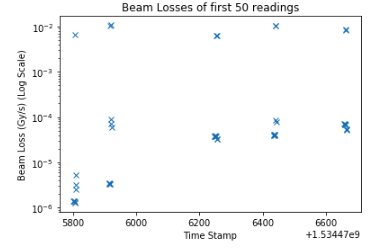
\includegraphics[width=\linewidth]{BLM1}
			\captionof{figure}{BLM losses at injection}
			\label{fig:BLMlosses}
		\end{minipage}%
		\begin{minipage}{.5\textwidth}
			\centering
			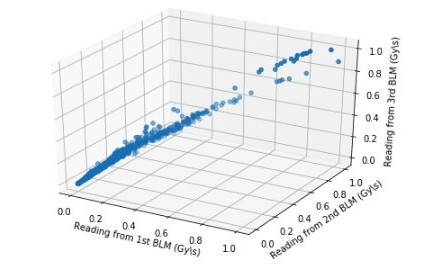
\includegraphics[width=\linewidth]{BLM2}
			\captionof{figure}{Normalised losses of 3 BLMs}
			\label{fig:BLMscatter}
		\end{minipage}
	\end{figure}
	
	
	\section{The Evaluation Strategy and Technique being Proposed}
	
	\section{Deliverables}
	
	\section{Progress}
	
	\begin{thebibliography}{14}
		\bibitem{r:BeamQC}
		V. Kain \textit{et. al} ``Injection beam loss and beam quality checks for the lhc." in \textit{Proc. IPAC}, 2010, pp. 1671-1673.
		
		\bibitem{r:Diagram}
		C. Lefevre. ``The cern accelerator complex." Technical report, 2008.
		
		\bibitem{r:LS}
		C. Roderick, L. Burdzanowski and G. Kruk. ``The cern accelerator logging service- 10 years in operation: a look at the past, present and future," presented at the 14\textsuperscript{th} Int. Conf. Accelerator \& Large Experimental Physics Control Systems, USA, 2013.
		
		\bibitem{r:AutomaticIQCChecks}
		L. N. Drosdal \textit{et. al.} ``Automatic injection quality checks for the lhc." in \textit{Proc. ICALEPCS}, 2011, pp. 1077-1080.
		
		\bibitem{r:CERNDocumentServer}
		``Cern document server" Internet: \texttt{cds.cern.ch}, [Nov. 11, 2018].
		
		\bibitem{r:lecturenotes}
		A. Hyv{\"a}rinen. Lecture Notes, Topic: ``Unsupervised machine learning." University of Helsinki, 2015.
		
		\bibitem{r:jin}
		J. Xin and H. Jiawei. ``K-means clustering." \textit{Encyclopaedia of Machine Learning}, pp. 563-564, 2011.
		
		\bibitem{r:DBSCAN}
		M. Ester \textit{et. al.} ``A density-based algorithm for discovering clusters in large spatial databases with noise." in \textit{Proc. KDD}, 1996, pp. 226-231.
		
		\bibitem{r:skclustering}
		``Clustering." Internet: \texttt{scikit-learn.org/stable/modules/clustering.html}, [Nov. 27, 2018].
		
		\bibitem{r:LOF}
		M. Breunig \textit{et. al.} ``Lof: identifying density-based local outliers," in \textit{Proc. ACM SIGMOD}, 2000, pp. 1-12.
		
		\bibitem{r:pymvpa}
		PyMVPA Authors. ``Pymvpa developer guidelines." Internet: \texttt{www.pymvpa.org}, Aug. 28, 2017 [Nov. 26, 2018].
		
		\bibitem{r:shogun}
		``The shogun machine learning toolbox." Internet: \texttt{pypi.org/project/shogun-ml/}, [Nov. 26, 2018].
		
		\bibitem{r:sklearn}
		F. Pendregosa \textit{et. al.}. ``Scikit learn: machine learning in python." \textit{Journal of Machine Learning Research}, vol. 12, pp. 2825-2830, Oct. 2011.
		
		\bibitem{r:BLMs}
		E. Barbara Holzer, \textit{et. al.} ``Beam loss monitoring system for the lhc." in \textit{Proc. IEEE NSS}, 2005. 
	\end{thebibliography}
\end{document}